\documentclass{standalone}
\usepackage{tikz}
\usetikzlibrary{patterns, positioning}


\begin{document}
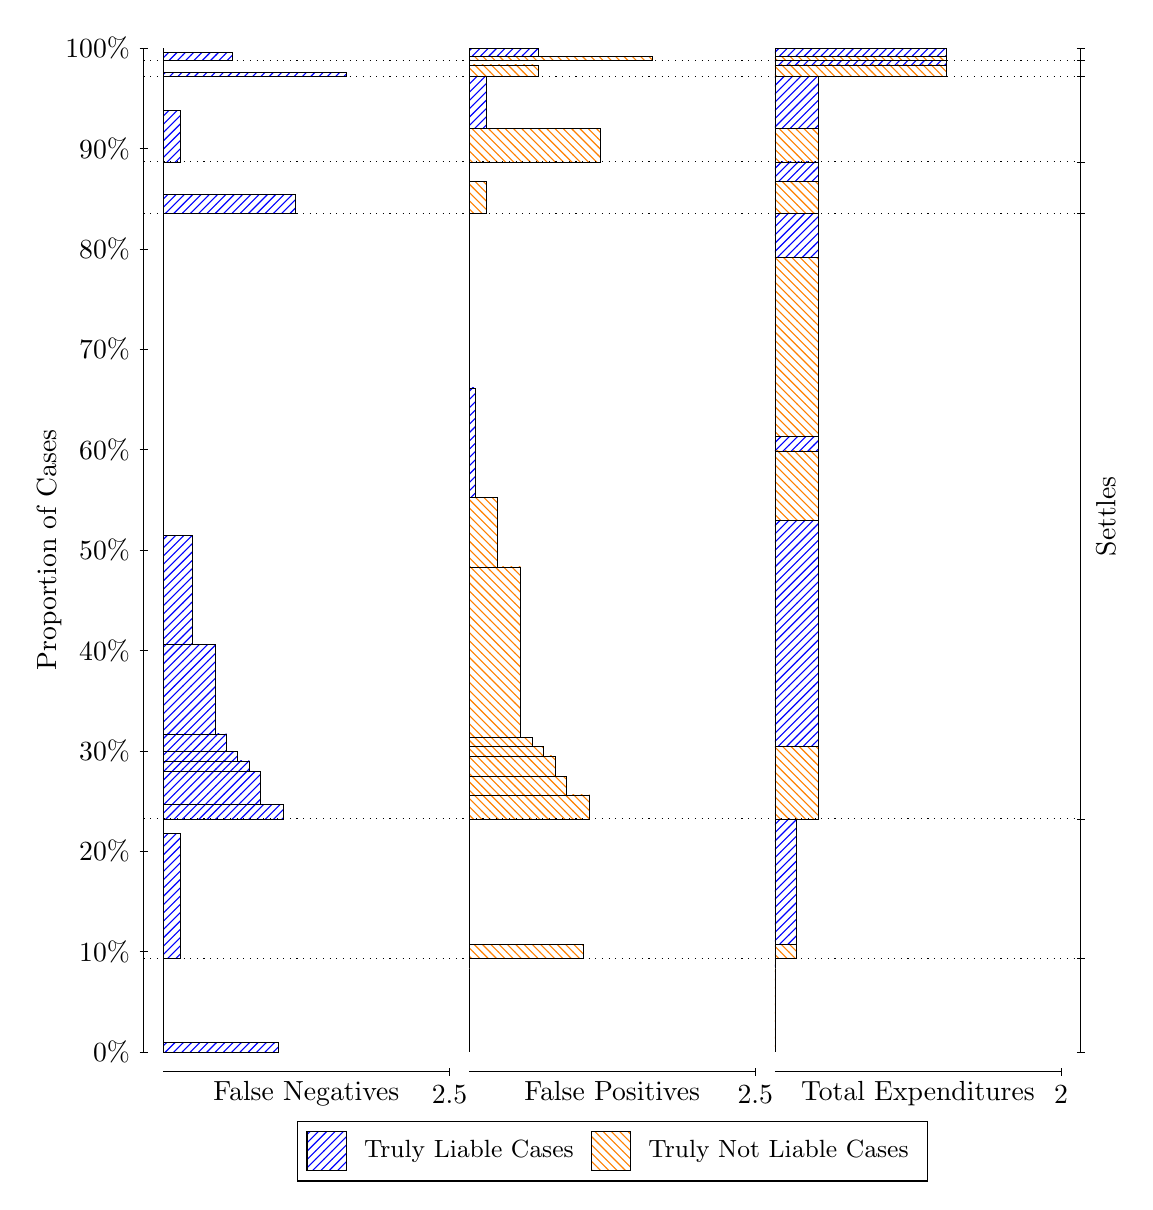
\begin{tikzpicture}
\draw[black, very thin] (1.5,1.75) -- (1.5,14.5);
\node[rotate=90, text=black, anchor=center] at (0.3, 8.125) {Proportion of Cases};
\draw[black, very thin] (1.45,1.75) -- (1.55,1.75);
\node[text=black, anchor=east] at (1.45, 1.75) {0\%};
\draw[black, very thin] (1.45,3.025) -- (1.55,3.025);
\node[text=black, anchor=east] at (1.45, 3.025) {10\%};
\draw[black, very thin] (1.45,4.3) -- (1.55,4.3);
\node[text=black, anchor=east] at (1.45, 4.3) {20\%};
\draw[black, very thin] (1.45,5.575) -- (1.55,5.575);
\node[text=black, anchor=east] at (1.45, 5.575) {30\%};
\draw[black, very thin] (1.45,6.85) -- (1.55,6.85);
\node[text=black, anchor=east] at (1.45, 6.85) {40\%};
\draw[black, very thin] (1.45,8.125) -- (1.55,8.125);
\node[text=black, anchor=east] at (1.45, 8.125) {50\%};
\draw[black, very thin] (1.45,9.4) -- (1.55,9.4);
\node[text=black, anchor=east] at (1.45, 9.4) {60\%};
\draw[black, very thin] (1.45,10.675) -- (1.55,10.675);
\node[text=black, anchor=east] at (1.45, 10.675) {70\%};
\draw[black, very thin] (1.45,11.95) -- (1.55,11.95);
\node[text=black, anchor=east] at (1.45, 11.95) {80\%};
\draw[black, very thin] (1.45,13.225) -- (1.55,13.225);
\node[text=black, anchor=east] at (1.45, 13.225) {90\%};
\draw[black, very thin] (1.45,14.5) -- (1.55,14.5);
\node[text=black, anchor=east] at (1.45, 14.5) {100\%};

\draw[black, very thin] (13.4,1.75) -- (13.4,14.5);
\draw[black, very thin] (13.35,1.75) -- (13.45,1.75);
\node[anchor=west] at (13.35, 1.75) {};
\draw[black, very thin] (13.35,2.9362) -- (13.45,2.9362);
\node[anchor=west] at (13.35, 2.9362) {};
\draw[black, very thin] (13.35,4.7111) -- (13.45,4.7111);
\node[anchor=west] at (13.35, 4.7111) {};
\draw[black, very thin] (13.35,12.397) -- (13.45,12.397);
\node[anchor=west] at (13.35, 12.397) {};
\draw[black, very thin] (13.35,13.055) -- (13.45,13.055);
\node[anchor=west] at (13.35, 13.055) {};
\draw[black, very thin] (13.35,14.135) -- (13.45,14.135);
\node[anchor=west] at (13.35, 14.135) {};
\draw[black, very thin] (13.35,14.34) -- (13.45,14.34);
\node[anchor=west] at (13.35, 14.34) {};
\draw[black, very thin] (13.35,14.5) -- (13.45,14.5);
\node[anchor=west] at (13.35, 14.5) {};

\draw[black, very thin, pattern color=blue, pattern=north east lines] (1.75,1.75) rectangle (3.2033,1.8748);
\draw[black, very thin, pattern color=orange, pattern=north west lines] (1.75,1.8748) rectangle (1.75,2.9362);
\draw[black, very thin, pattern color=blue, pattern=north east lines] (1.75,2.9362) rectangle (1.968,4.526);
\draw[black, very thin, pattern color=orange, pattern=north west lines] (1.75,4.526) rectangle (1.75,4.7111);
\draw[black, very thin, pattern color=blue, pattern=north east lines] (1.75,4.7111) rectangle (3.276,4.8924);
\draw[black, very thin, pattern color=blue, pattern=north east lines] (1.75,4.8924) rectangle (2.9853,5.316);
\draw[black, very thin, pattern color=blue, pattern=north east lines] (1.75,5.316) rectangle (2.84,5.4472);
\draw[black, very thin, pattern color=blue, pattern=north east lines] (1.75,5.4472) rectangle (2.6947,5.5679);
\draw[black, very thin, pattern color=blue, pattern=north east lines] (1.75,5.5679) rectangle (2.5493,5.7887);
\draw[black, very thin, pattern color=blue, pattern=north east lines] (1.75,5.7887) rectangle (2.404,6.9231);
\draw[black, very thin, pattern color=blue, pattern=north east lines] (1.75,6.9231) rectangle (2.1133,8.3142);
\draw[black, very thin, pattern color=orange, pattern=north west lines] (1.75,8.3142) rectangle (1.75,12.397);
\draw[black, very thin, pattern color=blue, pattern=north east lines] (1.75,12.397) rectangle (3.4213,12.641);
\draw[black, very thin, pattern color=orange, pattern=north west lines] (1.75,12.641) rectangle (1.75,13.055);
\draw[black, very thin, pattern color=blue, pattern=north east lines] (1.75,13.055) rectangle (1.968,13.708);
\draw[black, very thin, pattern color=orange, pattern=north west lines] (1.75,13.708) rectangle (1.75,14.135);
\draw[black, very thin, pattern color=blue, pattern=north east lines] (1.75,14.135) rectangle (4.0753,14.189);
\draw[black, very thin, pattern color=orange, pattern=north west lines] (1.75,14.189) rectangle (1.75,14.34);
\draw[black, very thin, pattern color=blue, pattern=north east lines] (1.75,14.34) rectangle (2.622,14.447);
\draw[black, very thin, pattern color=orange, pattern=north west lines] (1.75,14.447) rectangle (1.75,14.5);
\draw[black, very thin, pattern color=orange, pattern=north west lines] (5.6333,1.75) rectangle (5.6333,2.8114);
\draw[black, very thin, pattern color=blue, pattern=north east lines] (5.6333,2.8114) rectangle (5.6333,2.9362);
\draw[black, very thin, pattern color=orange, pattern=north west lines] (5.6333,2.9362) rectangle (7.0867,3.1212);
\draw[black, very thin, pattern color=blue, pattern=north east lines] (5.6333,3.1212) rectangle (5.6333,4.7111);
\draw[black, very thin, pattern color=orange, pattern=north west lines] (5.6333,4.7111) rectangle (7.1593,5.0139);
\draw[black, very thin, pattern color=orange, pattern=north west lines] (5.6333,5.0139) rectangle (6.8687,5.2487);
\draw[black, very thin, pattern color=orange, pattern=north west lines] (5.6333,5.2487) rectangle (6.7233,5.5111);
\draw[black, very thin, pattern color=orange, pattern=north west lines] (5.6333,5.5111) rectangle (6.578,5.6318);
\draw[black, very thin, pattern color=orange, pattern=north west lines] (5.6333,5.6318) rectangle (6.4327,5.7422);
\draw[black, very thin, pattern color=orange, pattern=north west lines] (5.6333,5.7422) rectangle (6.2873,7.9094);
\draw[black, very thin, pattern color=orange, pattern=north west lines] (5.6333,7.9094) rectangle (5.9967,8.7937);
\draw[black, very thin, pattern color=blue, pattern=north east lines] (5.6333,8.7937) rectangle (5.706,10.185);
\draw[black, very thin, pattern color=blue, pattern=north east lines] (5.6333,10.185) rectangle (5.6333,12.397);
\draw[black, very thin, pattern color=orange, pattern=north west lines] (5.6333,12.397) rectangle (5.8513,12.811);
\draw[black, very thin, pattern color=blue, pattern=north east lines] (5.6333,12.811) rectangle (5.6333,13.055);
\draw[black, very thin, pattern color=orange, pattern=north west lines] (5.6333,13.055) rectangle (7.3047,13.483);
\draw[black, very thin, pattern color=blue, pattern=north east lines] (5.6333,13.483) rectangle (5.8513,14.135);
\draw[black, very thin, pattern color=orange, pattern=north west lines] (5.6333,14.135) rectangle (6.5053,14.286);
\draw[black, very thin, pattern color=blue, pattern=north east lines] (5.6333,14.286) rectangle (5.6333,14.34);
\draw[black, very thin, pattern color=orange, pattern=north west lines] (5.6333,14.34) rectangle (7.9587,14.393);
\draw[black, very thin, pattern color=blue, pattern=north east lines] (5.6333,14.393) rectangle (6.5053,14.5);
\draw[black, very thin, pattern color=orange, pattern=north west lines] (9.5167,1.75) rectangle (9.5167,2.8114);
\draw[black, very thin, pattern color=blue, pattern=north east lines] (9.5167,2.8114) rectangle (9.5167,2.9362);
\draw[black, very thin, pattern color=orange, pattern=north west lines] (9.5167,2.9362) rectangle (9.7892,3.1212);
\draw[black, very thin, pattern color=blue, pattern=north east lines] (9.5167,3.1212) rectangle (9.7892,4.7111);
\draw[black, very thin, pattern color=orange, pattern=north west lines] (9.5167,4.7111) rectangle (10.062,5.6318);
\draw[black, very thin, pattern color=blue, pattern=north east lines] (9.5167,5.6318) rectangle (10.062,8.4988);
\draw[black, very thin, pattern color=orange, pattern=north west lines] (9.5167,8.4988) rectangle (10.062,9.3831);
\draw[black, very thin, pattern color=blue, pattern=north east lines] (9.5167,9.3831) rectangle (10.062,9.5644);
\draw[black, very thin, pattern color=orange, pattern=north west lines] (9.5167,9.5644) rectangle (10.062,11.842);
\draw[black, very thin, pattern color=blue, pattern=north east lines] (9.5167,11.842) rectangle (10.062,12.397);
\draw[black, very thin, pattern color=orange, pattern=north west lines] (9.5167,12.397) rectangle (10.062,12.811);
\draw[black, very thin, pattern color=blue, pattern=north east lines] (9.5167,12.811) rectangle (10.062,13.055);
\draw[black, very thin, pattern color=orange, pattern=north west lines] (9.5167,13.055) rectangle (10.062,13.483);
\draw[black, very thin, pattern color=blue, pattern=north east lines] (9.5167,13.483) rectangle (10.062,14.135);
\draw[black, very thin, pattern color=orange, pattern=north west lines] (9.5167,14.135) rectangle (11.697,14.286);
\draw[black, very thin, pattern color=blue, pattern=north east lines] (9.5167,14.286) rectangle (11.697,14.34);
\draw[black, very thin, pattern color=orange, pattern=north west lines] (9.5167,14.34) rectangle (11.697,14.393);
\draw[black, very thin, pattern color=blue, pattern=north east lines] (9.5167,14.393) rectangle (11.697,14.5);
\draw[black, dotted] (1.5,2.9362) -- (13.4,2.9362);
\draw[black, dotted] (1.5,4.7111) -- (13.4,4.7111);
\draw[black, dotted] (1.5,12.397) -- (13.4,12.397);
\draw[black, dotted] (1.5,13.055) -- (13.4,13.055);
\draw[black, dotted] (1.5,14.135) -- (13.4,14.135);
\draw[black, dotted] (1.5,14.34) -- (13.4,14.34);
\draw[black, very thin] (1.75,1.5) -- (5.3833,1.5);
\node[text=black, anchor=north] at (3.5667, 1.5) {False Negatives};
\draw[black, very thin] (5.3833,1.45) -- (5.3833,1.55);
\node[text=black, anchor=north] at (5.3833, 1.45) {2.5};

\draw[black, very thin] (5.6333,1.5) -- (9.2667,1.5);
\node[text=black, anchor=north] at (7.45, 1.5) {False Positives};
\draw[black, very thin] (9.2667,1.45) -- (9.2667,1.55);
\node[text=black, anchor=north] at (9.2667, 1.45) {2.5};

\draw[black, very thin] (9.5167,1.5) -- (13.15,1.5);
\node[text=black, anchor=north] at (11.333, 1.5) {Total Expenditures};
\draw[black, very thin] (13.15,1.45) -- (13.15,1.55);
\node[text=black, anchor=north] at (13.15, 1.45) {2};



\node[text=black, centered, rotate=90] at (13.72, 8.554) {Settles};





\draw (7.449999999999999,1.5) node[draw=none] (baseCoordinate) {};
\begin{scope}[align=center]
        \matrix[scale=0.5, draw=black, below=0.5cm of baseCoordinate, nodes={draw}, column sep=0.1cm]{
            \node[rectangle, draw, minimum width=0.5cm, minimum height=0.5cm, pattern color=blue, pattern=north east lines] {}; &
            \node[draw=none, font=\small, text=black] (B) {Truly Liable Cases}; &
            \node[rectangle, draw, minimum width=0.5cm, minimum height=0.5cm, pattern color=orange, pattern=north west lines] {}; &
            \node[draw=none, font=\small, text=black] (B) {Truly Not Liable Cases}; \\
            };
\end{scope}

\end{tikzpicture}
\end{document}